\chapter{Experimental} % Main chapter title
\label{Chapter5} 
\section{General Materials and Methods}
All reagents except novel compounds and Mallard Blue, were obtained from commercial sources and used without further purification unless otherwise stated. Mallard Blue was synthesised by a previously reported synthesis.\textsuperscript{\cite{Bromfield2013MallardMedia}}

Thin layer chromatography (TLC) was performed on Merck aluminium backed plates, coated with 0.25 nm silica gel 60.
\newline
Flash column chromatography was performed on silica gel 60 (35 – 70 \textmu m) supplied by Fluka Ltd.
\newline
NMR spectra were recorded on a JEOL ECX400 (\textsuperscript{1}H 400 MHz, \textsuperscript{13}C 100 MHz) spectrometer and assignments made through corroboration with DEPT-135 spectra.
\newline
ESI and HR mass spectra were recorded on a Bruker Daltonics MicroTOF mass spectrometer. 
\newline
IR spectroscopy was performed on a Perkin Elmer Spectrum Two FTIR spectrophotometer. 
\newline
UV-Visible spectroscopy was performed on a Shimadzu UV-2401PC spectrophotometer.
\newline
Fluorimetric assays (Nile Red, Ethidium Bromide) were performed using a Hitachi F4500 fluorimeter.
\newline
Transmission Electron Microscopy was performed using a FEI Tecnai 12 G2 electron microscope.
\newline
Dynamic Light Scattering was performed using a Malvern Zetasizer NanoSeries machine. 
\newline
Circular Dichroism was carried out on a Jasco
J810 CD Spectrophotometer (150w Xe lamp).

Where both enantiomers of a compound has been synthesised, synthesis of both enantiomers is identical to the L-enantiomer unless otherwise stated. 
Where melting points of compounds are \textbf{not} provided, this is due to insufficient compound remaining after other analysis techniques have been performed. 

\newpage
\section{Synthesis of Novel Self-Assembling Heparin Binders}
\subsection*{Synthesis of L-Lysine(Boc)\textsubscript{2} and D-Lysine(Boc)\textsubscript{2}}
\begin{figure} [h!]
\centering
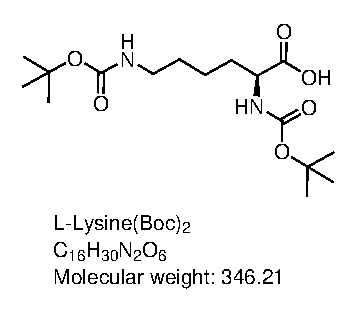
\includegraphics{Figures/L-Lys_boc_2.eps}
\end{figure}
L-lysine (2.10 g, 14.36 mmol) and  sodium hydroxide pellets (1.16 g, 29.00 mmol) were dissolved in deionised water (25 ml).   Di-tert-butyl dicarbonate (Boc anhydride) (6.25 g, 28.63 mmol) was dissolved separately into 25 ml THF.  The Boc anhydride solution was added dropwise over a period of 30 minutes into the basic L-lysine solution.  The reaction mixture was then heated to 45\textdegree C under a nitrogen atmosphere and stirred for three hours, before the solvent was removed \textit{in vacuo}. 
\newline
The remaining residue was dissolved in deionised water (100 ml) and washed with cyclohexane (50 ml), before the aqueous layer was acidified to pH 3 using 1.33M NaHSO\textsubscript{4} and the solvent removed in \textit{vacuo}.  The product is an hygroscopic, pale pink crystalline solid. (2.14g, 6.18 mmol,  43.05\%) D-lysine(Boc)\textsubscript{2} (4.40g, 12.70 mmol, 88.44\%)

Melting point: 44.4-45.8 \textdegree C,
D-Lysine(Boc)\textsubscript{2} 45.1-46.2 \textdegree C
\newline
R\textsubscript{f} = 0.51 (9:1, DCM:methanol, ninhydrin)
\newline
\textsuperscript{1}H NMR (400 MHz, CD\textsubscript{3}OD) \textdelta : 4.07-4.00 (m, C\textbf{H}NH, 1H); 3.89 (dd, C\textbf{H}\textsubscript{a}H\textsubscript{b}NH, 1H); 2.99 (t, C\textbf{H\textsubscript{2}}NH, \textit{\textsuperscript{3}J} = 6.6 Hz, 2H); 1.77-1.73 (m, C\textbf{H\textsubscript{a}}H\textsubscript{b}CHNH, 1H); 1.63-1.55 (m, CH\textsubscript{a}\textbf{H}\textsubscript{b}CHNH, 1H); 1.44 (br s, CH\textsubscript{2}C\textbf{H}\textsubscript{2}CH\textsubscript{2}NH, 2x C(C\textbf{H}\textsubscript{3})\textsubscript{3}, 24H); 1.26-1.17 (m, CH\textsubscript{2}C\textbf{H}\textsubscript{2}CH\textsubscript{2}NH, 1H)
\newline
\textsuperscript{13}C NMR (100 MHz, CD\textsubscript{3}OD) \textdelta :
176.4 (\textbf{C}OOH); 158.7 (\textbf{C}OONH); 158.3 (\textbf{C}OONH); 101.4, 80.6 (\textbf{C}(CH\textsubscript{3})\textsubscript{3}); 80.0 (\textbf{C}(CH\textsubscript{3})\textsubscript{3}); 54.9 (CH\textsubscript{2}\textbf{C}HNH); 41.1 (CH\textsubscript{2}\textbf{C}H\textsubscript{2}NH); 32.6 (\textbf{C}H\textsubscript{2}CHNH), 30.6 (\textbf{C}H\textsubscript{2}CH\textsubscript{2}NH, 29.0 (C(\textbf{C}H\textsubscript{3})\textsubscript{3} x3); 28.9 (C(\textbf{C}H\textsubscript{3})\textsubscript{3} x3); 24.2 (\textbf{C}H\textsubscript{2}CH\textsubscript{2}CH\textsubscript{2}NH).  
\newline
ESI-MS: 369.19 [M+Na]\textsuperscript{+} (90\%), 347.21 [M+H]\textsuperscript{+} (20\%)
\newline
HRMS: L-lysine(Boc)\textsubscript{2} Calcd.
[M+H]\textsuperscript{+} (C\textsubscript{16}H\textsubscript{31}N\textsubscript{2}O\textsubscript{6}) m/z = 347.2177, found [M+Na]\textsuperscript{+} m/z = 347.2170 (error 1.8 ppm)
\newline
[M+Na]\textsuperscript{+} (C\textsubscript{16}H\textsubscript{30}N\textsubscript{2}NaO\textsubscript{6}) m/z = 369.1996, found [M+Na]\textsuperscript{+} m/z = 369.1986 (error 3.4 ppm).
\newline
HRMS: D-lysine(Boc)\textsubscript{2} Calcd. 
[M+H]\textsuperscript{+} (C\textsubscript{16}H\textsubscript{31}N\textsubscript{2}O\textsubscript{6}) m/z = 347.2177, found [M+Na]\textsuperscript{+} m/z = 347.2182 (error - 0.2 ppm)
\newline
[M+Na]\textsuperscript{+} (C\textsubscript{16}H\textsubscript{30}N\textsubscript{2}NaO\textsubscript{6}) m/z = 369.1996, found [M+Na]\textsuperscript{+} m/z = 369.1993 (error 0.9 ppm).
\newline 
IR \textit{v} [cm\textsuperscript{-1}]: 3343\textit{br w} (N-H), 2977\textit{m} (C-H), 2934\textit{m} (C-H), 2869\textit{m} (C-H), 1683\textit{s} (CONH), 1520\textit{m}, 1517\textit{m} (CONH), 1452\textit{m}, 1413\textit{m}, 1392\textit{m}, 1366\textit{s}, 1249\textit{m}, 1160\textit{s}, 1049\textit{m}, 1019\textit{m}, 861\textit{m}.   
\newline

\subsection*{Synthesis of C\textsubscript{16}-L-Ala(Boc) and C\textsubscript{16}-D-Ala(Boc)}
\begin{figure}[h!]
\centering
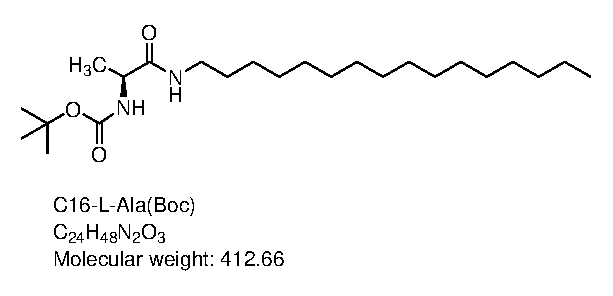
\includegraphics{Figures/C16-L-Ala_boc_.eps}
\end{figure}
L-Ala-(Boc)\textsubscript{2} (275 mg, 1.44 mmol) was dissolved in DCM (40 ml) before TBTU (463 mg, 1.44 mmol) and NEt\textsubscript{3} (5 ml) were added. 
The mixture was stirred for 5 minutes before 1-hexadecylamine (390 mg, 1.44 mmol) in DCM (20 ml) was added to the solution and left stirring overnight. 
The solvent was removed in \textit{vacuo} and the remaining residue redissolved in DCM (50 ml) before being washed with 1.33 M NaHSO\textsubscript{4} (2 x 15 ml), saturated NaHCO\textsubscript{3} (2 x 15 ml), water (3 x 15 ml) and saturated NaCl (15 ml). After purification by column chromatography, (SiO\textsubscript{2} in n-hexane: ethyl acetate 1:1) and solvent removed in \textit{vacuo}, the product was obtained as a white solid. (306 mg, 0.74 mmol, 51.47\%) C\textsubscript{16}-D-Ala(Boc) (398 mg, 0.97 mmol, 66.87\%)

R\textsubscript{f} = 0.73 (1:1, n-hexane: ethyl acetate, KMnO\textsubscript{4}) 
\newline
\textsuperscript{1}H NMR (400 MHz, CDCl\textsubscript{3}) \textdelta:
6.17 (br s, CH\textsubscript{3}CHCON\textbf{H}, 1H); 5.01 (br s, CHN\textbf{H}COOBoc, 1H); 4.12-4.08 (m, CH\textsubscript{3}C\textbf{H}NH, 1H);  3.24 (q, CONHC\textbf{H}\textsubscript{2}, \textit{\textsuperscript{3}J} = 6.4 Hz x3, 2H);  1.72 (s, C\textbf{H}\textsubscript{2}CH\textsubscript{2}NH, 2H); 1.48 (br d, CH\textsubscript{2}C\textbf{H}\textsubscript{2}CH\textsubscript{2}, \textit{\textsuperscript{3}J} = 6.4 Hz, 2H); 1.45 (d, C(C\textbf{H}3)\textsubscript{3},  9H); 1.36 (d, NHCH\textsubscript{2}C\textbf{H}\textsubscript{a}H\textsubscript{b}, \textit{\textsuperscript{3}J} = 1.92 Hz, 1H); 1.34 (br d,C\textbf{H}\textsubscript{3}CHCONH, \textsuperscript{3}J = 1.4 Hz, 3H); 1.26 (s, CH\textsubscript{2}C\textbf{H}\textsubscript{2}CH\textsubscript{2}, 24H); 0.89 (app t, CH\textsubscript{2}CH\textsubscript{2}C\textbf{H}\textsubscript{3}, \textit{\textsuperscript{3}J} = 3 Hz, 3H).
\newline
\textsuperscript{13}C NMR (100 MHz, CDCl\textsubscript{3}) \textdelta:
172.4 (\textbf{C}OOH); 155.6 (\textbf{C}OOH); 99.9; 80.1 (\textbf{C}(CH\textsubscript{3})\textsubscript{3}); 50.0 (CH\textsubscript{3}\textbf{C}HCONH); 39.5 (\textbf{C}H\textsubscript{2}NH); 31.9 (\textbf{C}H\textsubscript{2}CH\textsubscript{2}CH\textsubscript{3}); 29.7 (CH\textsubscript{2}\textbf{C}H\textsubscript{2}CH\textsubscript{2} x4); 29.6 (CH\textsubscript{2}\textbf{C}H\textsubscript{2}CH\textsubscript{2} x2); 29.6 (CH\textsubscript{2}\textbf{C}H\textsubscript{2}CH\textsubscript{2});  29.5 (CH\textsubscript{2}\textbf{C}H\textsubscript{2}CH\textsubscript{2} x2); 29.3 (CH\textsubscript{2}\textbf{C}H\textsubscript{2}CH\textsubscript{2}); 29.3 (CH\textsubscript{2}\textbf{C}H\textsubscript{2}CH\textsubscript{2}); 28.3 (C(\textbf{C}H\textsubscript{3})\textsubscript{3} x3); 26.8 (\textbf{C}H\textsubscript{2}CH\textsubscript{2}CH\textsubscript{2}NH); 22.7 (\textbf{C}H\textsubscript{2}CH\textsubscript{3}); 18.3 (\textbf{C}H\textsubscript{3}CHCONH); 14.1 (CH\textsubscript{2}\textbf{C}H\textsubscript{3}).
\newline
ESI-MS: 435.35 [M+Na]\textsuperscript{+} (100\%), 413.37 [M+H]\textsuperscript{+} (50\%).
\newline
HRMS: C\textsubscript{16}-L-Ala(Boc) Calcd. 
[M+H]\textsuperscript{+} (C\textsubscript{24}H\textsubscript{49}N\textsubscript{2}O\textsubscript{3}) m/z = 413.3738 , found [M+H]\textsuperscript{+} m/z = 413.3719 (error 4.4 ppm)
\newline
[M+Na]\textsuperscript{+} (C\textsubscript{24}H\textsubscript{48}N\textsubscript{2}NaO\textsubscript{3}) m/z = 435.3557, found [M+Na]\textsuperscript{+} m/z = 435.3535 (error 5.3 ppm).
\newline
HRMS: C\textsubscript{16}-D-Ala(Boc) Calcd. [M+Na]\textsuperscript{+} (C\textsubscript{24}H\textsubscript{48}N\textsubscript{2}NaO\textsubscript{3}) m/z = 435.3557, found [M+Na]\textsuperscript{+} m/z = 435.3546 (error 3.7 ppm).
\newline
IR \textit{v} [cm\textsuperscript{-1}]: 3344\textit{w} (N-H), 3317\textit{m} (N-H), 3261\textit{m} (N-H), 3075\textit{w} (C-H), 2983\textit{m} (C-H), 2956\textit{m} (C-H), 2917\textit{s} (C-H), 2848\textit{s} (C-H), 1734\textit{w} (C=O), 1713\textit{w} (C=O), 1687\textit{s} (CONH), 1650\textit{s} (CONH), 1613\textit{w}, 1553\textit{m}, 1532\textit{s} (CONH), 1469\textit{m}, 1454\textit{m}, 1384\textit{m}, 1365\textit{m}, 1322\textit{m}, 1250\textit{s}, 1214\textit{m}, 1172\textit{s}, 1115\textit{m}, 1067\textit{m}, 1040\textit{m}, 1026\textit{m}, 867\textit{m}. 

\newpage
\subsection*{Synthesis of C\textsubscript{16}-L-Ala and C\textsubscript{16}-D-Ala}
\begin{figure}[h!]
\centering
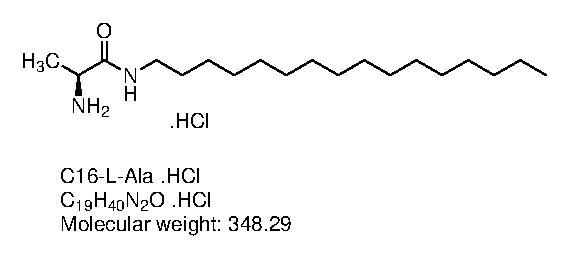
\includegraphics{Figures/C16-L-Ala.eps}
\end{figure}
C\textsubscript{16}-L-Ala(Boc) (146.20 mg, 0.35 mmol was dissolved in 4M HCl in dioxane (1.32 ml, 15 eq.) The solution was left stirring for 1 hour before the solvent was removed \textit{in vacuo} to give the product as a white foam. (90.81 mg, 0.26 mmol, 73.59\%) C\textsubscript{16}-D-Ala (325 mg, 0.93 mmol, 97.48\%)

\textsuperscript{1}H NMR (400 MHz, CD\textsubscript{3}OD) \textdelta :
3.89-3.84 (m, CH\textsubscript{3}C\textbf{H}CONH, 1H); 3.26-3.14 (m, C\textbf{H}\textsubscript{2}NH, 2H); 1.53-1.46 (m, C\textbf{H}\textsubscript{3}CHCONH + C\textbf{H}\textsubscript{2}CH\textsubscript{2}NH, 5H); 1.40-1.23 (m, CH\textsubscript{2}C\textbf{H}\textsubscript{2}CH\textsubscript{2}, 24H); 0.88 (br t, CH\textsubscript{2}C\textbf{H}\textsubscript{3}, \textit{\textsuperscript{3}J} = 6.3 Hz, 3H).
\newline
\textsuperscript{13}C NMR (100 MHz, CD\textsubscript{3}OD) \textdelta: 170.9 (\textbf{C}ONH); 101.5, 50.4 (CH\textsubscript{3}\textbf{C}HNH\textsubscript{2}); 40.8 (CH\textsubscript{2}\textbf{C}H\textsubscript{2}NH); 33.2 (\textbf{C}H\textsubscript{2}CH\textsubscript{2}CH\textsubscript{3}); 30.9, 30.9,  30.8, 30.6, 30.6,  30.5, all (CH\textsubscript{2}\textbf{C}H\textsubscript{2}CH\textsubscript{2} x 11); 28.1 (\textbf{C}H\textsubscript{2}CH\textsubscript{2}CH\textsubscript{2}NH); 23.9 (\textbf{C}H\textsubscript{2}CH\textsubscript{3}); 17.9 (\textbf{C}H\textsubscript{3}CHNH\textsubscript{2}); 14.6 (CH\textsubscript{2}\textbf{C}H\textsubscript{3}). 
\newline
ESI-MS: 335.30 [M+Na]\textsuperscript{+} (20\%), 313.32 [M+H]\textsuperscript{+} (100\%).
\newline
HRMS: C\textsubscript{16}-L-Ala Calcd. 
[M+H]\textsuperscript{+} (C\textsubscript{19}H\textsubscript{41}N\textsubscript{2}O) m/z = 313.3213, found [M+H]\textsuperscript{+} m/z = 313.3209 (error 2.3 ppm).
\newline
[M+Na]\textsuperscript{+} (C\textsubscript{19}H\textsubscript{40}N\textsubscript{2}NaO) m/z = 335.3033, found [M+Na]\textsuperscript{+} m/z = 335.3033 (error - 0.8 ppm).
\newline
HRMS: C\textsubscript{16}-D-Ala  Calcd. [M+H]\textsuperscript{+} (C\textsubscript{19}H\textsubscript{41}N\textsubscript{2}O) m/z = 313.3213, found [M+H]\textsuperscript{+} m/z = 313.3208 (error 0.2 ppm).
\newline
IR \textit{v} [cm\textsuperscript{-1}]:  3346\textit{w} (N-H), 3318\textit{m} (N-H), 3261\textit{w} (N-H), 2985\textit{w} (C-H), 2956\textit{m} (C-H), 2917\textit{s} (C-H), 2849\textit{s} (C-H), 1689\textit{s} (CONH), 1676\textit{m} (CONH), 1652\textit{s} (CONH), 1526\textit{s} (CONH), 1471\textit{s}, 144\textit{m}, 1365\textit{m}, 1320\textit{m}, 1250\textit{m}, 1229\textit{m}, 1170\textit{m}, 1125\textit{m}, 1065\textit{m}, 1031\textit{m}, 955\textit{w}, 934\textit{w}, 896\textit{w}, 860\textit{m},
\newpage
\subsection*{Synthesis of C\textsubscript{16}-L-Ala-L-Lys(Boc)\textsubscript{2} and C\textsubscript{16}-D-Ala-D-Lys(Boc)\textsubscript{2}}
\begin{figure}[h!]
\centering
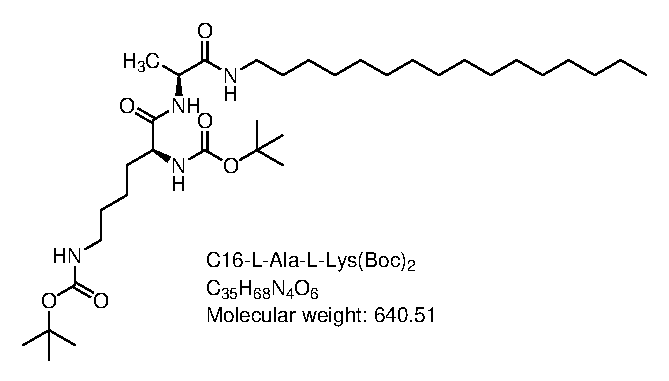
\includegraphics{Figures/C16-L-Ala-L-Lys_boc_2.eps}
\end{figure}
L-Lys(Boc)\textsubscript{2} (101 mg, 0.29 mmol) was dissolved in DCM (40 ml) before TBTU (93 mg, 0.29 mmol) and NEt\textsubscript{3} (5 ml) were added. The solution was left stirring for 5 minutes before C\textsubscript{16}-L-Ala (91 mg, 0.26 mmol) in DCM (20 ml) was added. The solution was left stirring overnight, before solvent was removed in \textit{vacuo}.
\newline
The remaining residue was redissolved in DCM (50 ml) before being washed with 1.33 M NaHSO\textsubscript{4} (2 x 15 ml), saturated NaHCO\textsubscript{3} (2 x 15 ml), water (3 x 15 ml) and saturated NaCl (15 ml). The solvent was removed in \textit{vacuo}, and the product obtained as a pale orange solid. (150 mg, 0.23 mmol, 88.46\%) C\textsubscript{16}-D-Ala-D-Lys(Boc)\textsubscript{2} pale yellow solid (151 mg, 0.24 mmol, 90.67\%)

\textsuperscript{1}H NMR (400 MHz, CDCl\textsubscript{3}) \textdelta:
6.71-6.47 (br s, CH\textsubscript{2}N\textbf{H}COOBoc + CHN\textbf{H}COOBoc, 2H) 5.58-5.43 (m, CH\textsubscript{2}N\textbf{H}COCH, 1H); 4.72 (br s, CON\textbf{H}CHCO, 1H); 4.43 (quint., CH\textsubscript{3}C\textbf{H}NHCONH,\textit{ \textsuperscript{3}J} = 7.2 Hz x4, 1H); 4.00 (br d, CH\textsubscript{2}C\textbf{H}NHCOOBoc, \textit{\textsuperscript{3}J} = 4.1 Hz, 1H); 3.31-3.18 (m, CH\textsubscript{2}C\textbf{H}\textsubscript{2}NHCOOBoc, 2H);
3.18-3.05 (m, CH\textsubscript{2}C\textbf{H}\textsubscript{2}NHCOCH, 2H); 1.76 (br s, C\textbf{H}\textsubscript{2}CHNH, 2H); 1.58-1.48 (m, C\textbf{H}\textsubscript{2}CH\textsubscript{2}NHCO, 4H); 1.46-1.43 (m, COOC(C\textbf{H}\textsubscript{3})\textsubscript{3}, 18H); 1.37 (d, C\textbf{H}\textsubscript{3}CHCONH, \textit{\textsuperscript{3}J}= 7.2 Hz, 3H); 1.36-1.31 (m, C\textbf{H}\textsubscript{2}CH\textsubscript{2}CH, 2H); 1.30-1.21 (m, CH\textsubscript{2}C\textbf{H}\textsubscript{2}CH\textsubscript{2}, 24H);  0.91-0.85 (m, CH\textsubscript{2}C\textbf{H}\textsubscript{3}, 3H).     
\newline
\textsuperscript{13}C NMR (100 MHz, CDCl\textsubscript{3}) \textdelta:
171.8 (CH\textbf{C}ONH); 166.9 (CH\textsubscript{3}CH\textbf{C}ONH); 157.3 (\textbf{C}OONH); 156.6 (\textbf{C}OONH); 80.5 (\textbf{C}(CH\textsubscript{3})\textsubscript{3} x2); 53.9 (CH\textsubscript{2}\textbf{C}HNH); 48.9 (CH\textsubscript{3}\textbf{C}HNH); 39.7 (CH\textsubscript{2}\textbf{C}H\textsubscript{2}NH); 38.6 (CH\textsubscript{2}\textbf{C}H\textsubscript{2}NH); 31.9 (\textbf{C}H\textsubscript{2}CH\textsubscript{2}CH\textsubscript{3}); 29.7 (\textbf{C}H\textsubscript{2}CH\textsubscript{2}NH); 29.6 (\textbf{C}H\textsubscript{2}CH\textsubscript{2}CH\textsubscript{2} x4); 29.6 (CH\textsubscript{2}\textbf{C}H\textsubscript{2}CH\textsubscript{2} x2); 29.5 (CH\textsubscript{2}\textbf{C}H\textsubscript{2}CH\textsubscript{2}); 29.3 (CH\textsubscript{2}\textbf{C}H\textsubscript{2}CH\textsubscript{2} x2); 29.3 (CH\textsubscript{2}\textbf{C}H\textsubscript{2}CH\textsubscript{2}); 28.5  (C(\textbf{C}H\textsubscript{3})\textsubscript{3} x3);  28.3 (C(\textbf{C}H\textsubscript{3})\textsubscript{3} x3); 26.8 (\textbf{C}H\textsubscript{2}CH\textsubscript{2}CH\textsubscript{2}NH); 22.7 (\textbf{C}H\textsubscript{2}CH\textsubscript{3}); 22.2 (\textbf{C}H\textsubscript{2}CH\textsubscript{2}CHNH); 18.1 (CH\textbf{C}H\textsubscript{3}); 14.1 (CH\textsubscript{2}\textbf{C}H\textsubscript{3}). 
\newline
ESI-MS: 663.50 [M+Na]\textsuperscript{+} (100\%).
\newline
HRMS: C\textsubscript{16}-L-Ala-L-Lys(Boc)\textsubscript{2} Calcd. [M+Na]\textsuperscript{+} (C\textsubscript{35}H\textsubscript{68}N\textsubscript{4}NaO\textsubscript{6}) m/z = 663.5031, found [M+Na]\textsuperscript{+} m/z = 663.5044 (error -1.9 ppm).
HRMS: C\textsubscript{16}-D-Ala-D-Lys(Boc)\textsubscript{2} Calcd. [M+H]\textsuperscript{+} (C\textsubscript{35}H\textsubscript{68}N\textsubscript{4}O\textsubscript{6}) m/z = 641.5390, found [M+H]\textsuperscript{+} m/z = 641.5212.
\newline
IR \textit{v} [cm\textsuperscript{-1}]: 3293\textit{br m} (N-H), 2919\textit{m} (C-H), 2851\textit{m} (C-H), 1686\textit{m} (CONH), 1643\textit{s} (CONH), 1525\textit{s} (CONH), 1467\textit{m}, 1454\textit{m}, 1365\textit{m}, 1273\textit{m}, 1247\textit{m}, 1168\textit{s}, 1102\textit{w}, 1048\textit{m}, 966\textit{w}, 923\textit{w}, 867\textit{w}.  
\newline

\subsection*{Synthesis of C\textsubscript{16}-D-Ala-L-Lys(Boc)\textsubscript{2} and C\textsubscript{16}-L-Ala-D-Lys(Boc)\textsubscript{2}}
\begin{figure}[h!]
\centering
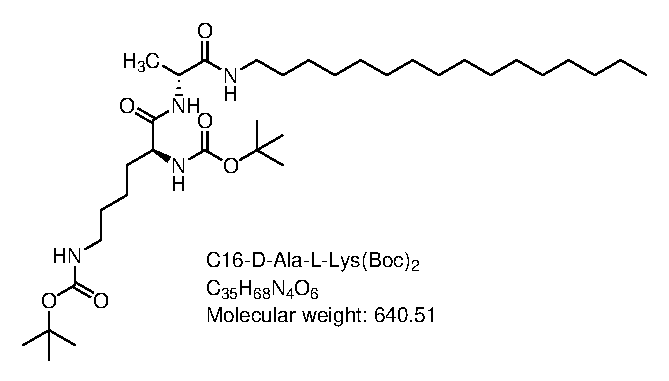
\includegraphics{Figures/C16-D-Ala-L-Lys_boc_2.eps}
\end{figure}
L-Lys(Boc)\textsubscript{2} (348 mg, 1.005 mmol) was dissolved in DCM (40 ml) before TBTU (323 mg, 1.005 mmol) and NEt\textsubscript{3} (9 ml) were added. The solution was left stirring for 5 minutes before C\textsubscript{16}-D-Ala (314 mg, 0.90 mmol)  in DCM (20 ml) was added. The solution was left stirring overnight, before solvent was removed in \textit{vacuo}.
\newline
The  remaining residue was redissolved in DCM (50 ml) before being washed with 1.33 M NaHSO\textsubscript{4} (2 x 25 ml), saturated NaHCO\textsubscript{3} (2 x 25 ml), water (3 x 25 ml) and saturated NaCl (25 ml). The solvent was removed in \textit{vacuo}, and the product obtained as a pale orange solid. (340 mg, 0.53 mmol, 58.98\%)  C\textsubscript{16}-L-Ala-D-Lys(Boc)\textsubscript{2} (152 mg, 0.31 mmol, 86.36\%). 

\textsuperscript{1}H NMR (400 MHz, CCl\textsubscript{3}) \textdelta:  
6.64-6.47 (br s, CH\textsubscript{2}N\textbf{H}COOBoc + CHN\textbf{H}COOBoc, 2H); 5.24-5.17 (m, CH\textsubscript{2}N\textbf{H}COCH, 1H); 4.67-4.60 (m, CON\textbf{H}CHCO, 1H); 4.48-4.39 (m, CH\textsubscript{3}C\textbf{H}NHCONH, 1H); 4.04-3.93 (m, CH\textsubscript{2}C\textbf{H}NHCOOBoc, 1H); 3.30-3.17 (m, CH\textsubscript{2}C\textbf{H}\textsubscript{2}NHCOOBoc, 2H);
3.17-3.08 (m,CH\textsubscript{2}C\textbf{H}\textsubscript{2}NHCOCH, 2H); 1.70-1.68 (br s, C\textbf{H}\textsubscript{2}CHNH, 2H); 1.58-1.48 (m, C\textbf{H}\textsubscript{2}CH\textsubscript{2}NHCO, 4H); 1.47-1.43 (m, COOC(C\textbf{H}\textsubscript{3})\textsubscript{3}, 18H); 1.37 (d, C\textbf{H}\textsubscript{3}CHCONH, \textit{\textsuperscript{3}J}= 7.2 Hz, 3H); 1.25 (br d, CH\textsubscript{2}C\textbf{H}\textsubscript{2}CH\textsubscript{2}, \textit{\textsuperscript{3}J} = 1.8 Hz, 22H);  0.91-0.86 (m, CH\textsubscript{2}C\textbf{H}\textsubscript{3}, 3H)
\newline
\textsuperscript{13}C NMR (100 MHz, CCl\textsubscript{3}) \textdelta:
171.6 (CH\textbf{C}ONH); 170.5 (CH\textsubscript{3}CH\textbf{C}ONH); 167.3 (\textbf{C}OONH); 166.2 (\textbf{C}OONH); 78.8 (C(CH\textsubscript{3})\textsubscript{3} x2); 50.9 (CH\textsubscript{2}\textbf{C}HNH); 48.9 (CH\textsubscript{3}\textbf{C}HNH); 39.7 (CH\textsubscript{2}\textbf{C}H\textsubscript{2}NH); 38.9 (CH\textsubscript{2}\textbf{C}H\textsubscript{2}NH); 31.9 (\textbf{C}H\textsubscript{2}CH\textsubscript{2}CH\textsubscript{3}); 29.7 (\textbf{C}H\textsubscript{2}CH\textsubscript{2}NH); 29.70 (CH\textsubscript{2}\textbf{C}H\textsubscript{2}CH\textsubscript{2}); 29.6 (CH\textsubscript{2}\textbf{C}H\textsubscript{2}CH\textsubscript{2} x4); 29.5 (CH\textsubscript{2}\textbf{C}H\textsubscript{2}CH\textsubscript{2} x2); 29.5 (CH\textsubscript{2}\textbf{C}H\textsubscript{2}CH\textsubscript{2}); 29.4 (CH\textsubscript{2}\textbf{C}H\textsubscript{2}CH\textsubscript{2} x2); 29.2 (CH\textsubscript{2}\textbf{C}H\textsubscript{2}CH\textsubscript{2}); 28.4 (C(\textbf{C}H\textsubscript{3})\textsubscript{3} x3); 28.3 (C(\textbf{C}H\textsubscript{3})\textsubscript{3} x3); 26.9 (\textbf{C}H\textsubscript{2}CH\textsubscript{2}CH\textsubscript{2}NH); 22.7 (\textbf{C}H\textsubscript{2}CH\textsubscript{3}); 22.5 (\textbf{C}H\textsubscript{2}CH\textsubscript{2}CHNH); 18.2 (CH\textbf{C}H\textsubscript{3}); 14.1 (CH\textsubscript{2}\textbf{C}H\textsubscript{3}). 
\newline
ESI-MS:  663.50 [M+Na]\textsuperscript{+} (100\%), 641.52 [M+H]\textsuperscript{+} (10\%)
\newline
HRMS: C\textsubscript{16}-D-Ala-L-Lys(Boc)\textsubscript{2} Calcd. 
[M+H]\textsuperscript{+} (C\textsubscript{35}H\textsubscript{69}N\textsubscript{4}O\textsubscript{6}) m/z = 641.52116, found [M+H]\textsuperscript{+} m/z = 641.51812 (error 4.0 ppm),
\newline
[M+Na]\textsuperscript{+} (C\textsubscript{35}H\textsubscript{68}N\textsubscript{4}NaO\textsubscript{6}) m/z = 663.5031, found [M+Na]\textsuperscript{+} m/z = 663.5020 (error 2.2 ppm).
\newline
HRMS: C\textsubscript{16}-L-Ala-D-Lys(Boc)\textsubscript{2} Calcd. [M+Na]\textsuperscript{+} (C\textsubscript{35}H\textsubscript{68}N\textsubscript{4}NaO\textsubscript{6}) m/z = 663.5031, found [M+Na]\textsuperscript{+} m/z = 663.5028 (error 0.3 ppm).
\newline
IR \textit{v} [cm\textsuperscript{-1}]: 3292\textit{br m} (N-H), 2919\textit{m} (C-H), 2851\textit{m} (C-H), 1687\textit{m} (CONH), 1657\textit{m} (CONH), 1639\textit{s} (CONH), 1520\textit{m} (CONH), 1454\textit{m}, 1391\textit{m}, 1365\textit{m}, 1271\textit{m}, 1245\textit{s}, 1168\textit{s}, 1056\textit{m}, 868\textit{m}. 
\newline

\newpage
\subsection*{Synthesis of C\textsubscript{16}-L-Ala-L-Lys}
\begin{figure}[ht!]
\centering
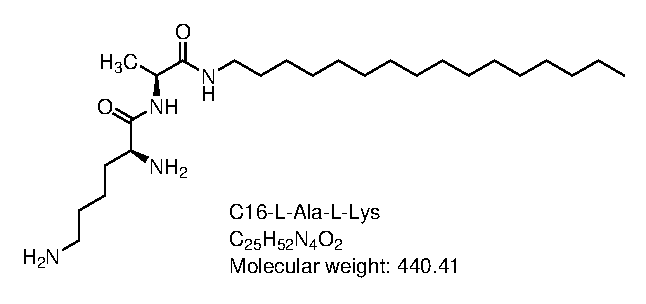
\includegraphics{Figures/C16-L-Ala-L-Lys.eps}
\end{figure}
C\textsubscript{16}-L-Ala-L-Lys(Boc)\textsubscript{2} (143 mg, 0.22 mmol) was dissolved in methanol, before HCl gas was bubbled through the solution for 30 seconds and stirred for 3 hours. The solvent was removed in \textit{vacuo} to afford the product as a bright orange solid. 40 mg, 0.09 mmol, 41.20\% yield. 

Melting point: 257.2-263.6 \textdegree C
\newline
\textsuperscript{1}H NMR (400 MHz, CD\textsubscript{3}OD) \textdelta: 4.32 (br d, CH\textsubscript{3}C\textbf{H}CONH, \textsuperscript{3}J= 7.3 Hz,  1H); 3.91 (br t,   CH\textsubscript{2}C\textbf{H}NH\textsubscript{2},\textit{\textsuperscript{3}J} = 6.2 Hz, 1H); 3.23-3.15 (m, C\textbf{H}\textsubscript{a}H\textsubscript{b}NHCOCH, 1H); 3.15-3.08 (m, CH\textsubscript{a}\textbf{H}\textsubscript{b}NHCOCH, 1H); 2.96 (br t, CH\textsubscript{2}C\textbf{H}\textsubscript{2}NH\textsubscript{2}, \textit{\textsuperscript{3}J} = 6.9 Hz, 2H); 1.91-1.86 (m, C\textbf{H}\textsubscript{2}CHNH, 2H); 1.73 - 1.67 (br s, C\textbf{H}\textsubscript{2}CH\textsubscript{2}CHNH\textsubscript{2}, 2H); 1.50-1.44 (m, C\textbf{H}\textsubscript{2}CH\textsubscript{2}NH\textsubscript{2}, 2H); 1.36-1.31 (m, C\textbf{H}\textsubscript{3}CHCONH, 3H); 1.26 (s, CH\textsubscript{2}C\textbf{H}\textsubscript{2}CH\textsubscript{2}, 18H);  0.87-0.85 (m, CH\textsubscript{2}C\textbf{H}\textsubscript{3}, 3H).
\newline
\textsuperscript{13}C NMR (100 MHz, CD\textsubscript{3}OD) \textdelta:
174.7 (CH\textbf{C}ONH); 169.8 (CH\textsubscript{3}\textbf{C}HCONH); 54.0 (CH\textsubscript{2}\textbf{C}HNH\textsubscript{2}); 50.8 (\textbf{C}HCH\textsubscript{3}); 40.7 (CH\textsubscript{2}\textbf{C}H\textsubscript{2}NH\textsubscript{2}); 40.4 (CH\textsubscript{2}\textbf{C}H\textsubscript{2}NH); 33.2 (\textbf{C}H\textsubscript{2}CHNH\textsubscript{2}); 32.1 (\textbf{C}H\textsubscript{2}CH\textsubscript{2}CH\textsubscript{3}); 30.9, 30.9, 30.6, 30.6 ( all CH\textsubscript{2}\textbf{C}H\textsubscript{2}CH\textsubscript{2} x 11); 30.5 (\textbf{C}H\textsubscript{2}CH\textsubscript{2}NH); 28.1 (\textbf{C}H\textsubscript{2}CH\textsubscript{2}CH\textsubscript{2}NH); 23.9 (\textbf{C}H\textsubscript{2}CH\textsubscript{3}); 22.5 (CH\textsubscript{2}\textbf{C}H\textsubscript{2}NH\textsubscript{2}); 18.5 (CH\textbf{C}H\textsubscript{3}); 14.6 (CH\textsubscript{2}\textbf{C}H\textsubscript{3});  
\newline
ESI-MS: 441.41 [M+H]\textsuperscript{+} (100\%).
\newline
HRMS: Calcd. [M+H]\textsuperscript{+} (C\textsubscript{25}H\textsubscript{53}N\textsubscript{4}O\textsubscript{2}) m/z = 441.4163, found [M+H]\textsuperscript{+} m/z = 441.4151 (error 3.2 ppm).
\newline
IR \textit{v} [cm\textsuperscript{-1}]: 3392\textit{br w} (N-H), 2919\textit{m} (C-H), 2851\textit{m} (C-H), 1662\textit{m} (CONH), 1639\textit{s} (CONH), 1563\textit{m}, 1558\textit{m} (CONH), 1464\textit{s}, 1376\textit{m}, 1293\textit{w}, 1286\textit{w}, 1255\textit{w}, 1153\textit{m}, 1072\textit{w}, 976\textit{w}, 948\textit{w}, 888\textit{w}.    
\newpage
\subsection*{Synthesis of C\textsubscript{16}-D-Ala-L-Lys and  C\textsubscript{16}-L-Ala-D-Lys }
\begin{figure}[ht!]
\centering
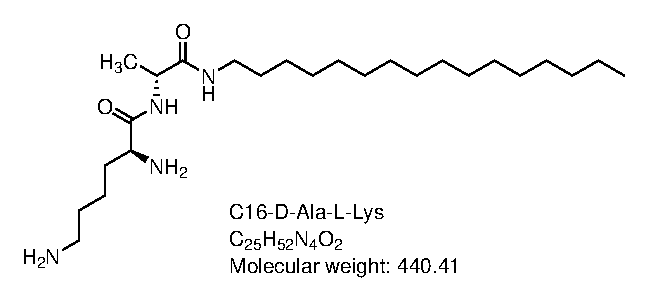
\includegraphics{Figures/C16-D-Ala-L-Lys.eps}
\end{figure}
C\textsubscript{16}-D-Ala-L-Lys(Boc)\textsubscript{2} (329 mg, 0.51 mmol) was dissolved in 4 M HCl in dioxane (1.92 ml, 15 eq). The solution was stirred at room temperature for 1 hour. The solvent was removed in \textit{vacuo} to afford the product as an off-white solid. (270 mg, 0.42 mmol, 82.35\%) C\textsubscript{16}-L-Ala-D-Lys 152 mg, 0.34 mmol, 81.17\%). 

Melting point: 255.8-260.5 \textdegree C, C\textsubscript{16}-L-Ala-D-Lys 255.6-260.8 \textdegree C
\newline
\textsuperscript{1}H NMR (400 MHz, CD\textsubscript{3}OD) \textdelta:  
4.34-4.28 (m, CH\textsubscript{3}C\textbf{H}CONH, 1H); 3.94-3.91 (m, CH\textsubscript{2}C\textbf{H}NH\textsubscript{2}, 1H); 3.19-3.15 (m, C\textbf{H}\textsubscript{2}NHCO, 2H); 2.97-2.93 (m, CH\textsubscript{2}C\textbf{H}\textsubscript{2}NH\textsubscript{2}, 2H); 1.91-1.80 (m, CH\textsubscript{2}C\textbf{H}\textsubscript{2}CHNH\textsubscript{2}, 2H); 1.74-1.70 (m, C\textbf{H}\textsubscript{2}CH\textsubscript{2}CHNH\textsubscript{2}, 2H); 1.49 (br d CH\textsubscript{2}C\textbf{H}\textsubscript{2}NH\textsubscript{2}, 2H); 1.39 (d, C\textbf{H}\textsubscript{3}CHCONH, \textit{\textsuperscript{3}J} = 7.3 Hz, 3H); 1.26 (br s, CH\textsubscript{2}C\textbf{H}\textsubscript{2}CH\textsubscript{2}, 24H);  0.91-0.84 (m, app t, CH\textsubscript{2}C\textbf{H}\textsubscript{3}, 3H).     
\newline
\textsuperscript{13}C NMR (100 MHz, CD\textsubscript{3}OD) \textdelta:
173.3 (CH\textbf{C}ONH); 169.9 (CH\textsubscript{3}\textbf{C}HCONH); 54.4 (CH\textsubscript{2}\textbf{C}HNH\textsubscript{2}); 50.9 (\textbf{C}HCH\textsubscript{3}); 40.7 (CH\textsubscript{2}\textbf{C}H\textsubscript{2}NH\textsubscript{2}); 40.4 (CH\textsubscript{2}\textbf{C}H\textsubscript{2}NH); 33.2 (\textbf{C}H\textsubscript{2}CHNH\textsubscript{2}); 32.1 (\textbf{C}H\textsubscript{2}CH\textsubscript{2}CH\textsubscript{3}); 30.9, 30.9, 30.8, 30.6 (all CH\textsubscript{2}\textbf{C}H\textsubscript{2}CH\textsubscript{2} x 11); 30.5 (\textbf{C}H\textsubscript{2}CH\textsubscript{2}NH); 28.3 (\textbf{C}H\textsubscript{2}CH\textsubscript{2}CH\textsubscript{2}NH); 23.9 (\textbf{C}H\textsubscript{2}CH\textsubscript{3}); 23.2 (CH\textsubscript{2}\textbf{C}H\textsubscript{2}NH\textsubscript{2}); 18.6 (CH\textbf{C}H\textsubscript{3}); 14.6 (CH\textsubscript{2}\textbf{C}H\textsubscript{3});  
\newline
ESI-MS: 441.41 [M+H]\textsuperscript{+} (100\%) 
\newline
HRMS: C\textsubscript{16}-D-Ala-L-Lys Calcd. [M+H]\textsuperscript{+} (C\textsubscript{25}H\textsubscript{53}N\textsubscript{4}O\textsubscript{2}) m/z = 441.4163, found [M+H]\textsuperscript{+} m/z = 441.4175 (error -2.9 ppm).
\newline
HRMS: C\textsubscript{16}-L-Ala-D-Lys Calcd. [M+H]\textsuperscript{+} (C\textsubscript{25}H\textsubscript{53}N\textsubscript{4}O\textsubscript{2}) m/z = 441.4163, found [M+H]\textsuperscript{+} m/z = 441.4148 (error 4.8 ppm).
\newline
IR \textit{v} [cm\textsuperscript{-1}]: 3398\textit{br w} (N-H), 2955\textit{w} (C-H), 2917\textit{m} (C-H), 2850\textit{m} (C-H), 1638\textit{s} (CONH), 1557\textit{w} (CONH), 1467\textit{s}, 1376\textit{m}, 1271\textit{w}, 1254\textit{w}, 1234\textit{w}, 1213\textit{m}, 1160\textit{m}, 1056\textit{m}, 979\textit{w}.
\newline

\newpage
\subsection*{Synthesis of C\textsubscript{16}-D-Ala-D-Lys}
\begin{figure}[ht!]
\centering
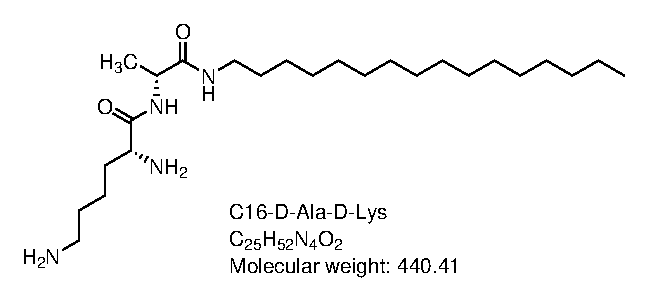
\includegraphics{Figures/C16-D-Ala-D-Lys.eps}
\end{figure}
C\textsubscript{16}-D-Ala-D-Lys(Boc)\textsubscript{2} (141 mg, 0.22 mmol) was dissolved in 4 M HCl in dioxane (0.82 ml, 15 eq). The solution was stirred at room temperature for 1 hour. The solvent was removed in \textit{vacuo} to afford the product as an of-white solid. (112 mg, 0.25 mmol, 95.00\%) 

Melting point: 261.7-263.7 \textdegree C
\newline
\textsuperscript{1}H NMR (400 MHz, CD\textsubscript{3}OD) \textdelta:  4.35-4.21 (m, CH\textsubscript{3}C\textbf{H}NH, 1H); 3.93-3.82 (m, CH\textsubscript{2}C\textbf{H}NH\textsubscript{2}, 1H); 3.21-3.00 (m CH\textsubscript{2}C\textbf{H}\textsubscript{2}NH, 2H); 2.98-2.84 (m, CH\textsubscript{2}C\textbf{H}\textsubscript{2}NH\textsubscript{2}, 2H); 1.92-1.78 (m, C\textbf{H}\textsubscript{2}CHNH\textsubscript{2}, 2H); 1.74-1.61 (m, C\textbf{H}\textsubscript{2}CH\textsubscript{2}CH\textsubscript{2}NH\textsubscript{2}, 2H); 1.58-1.41 (m, C\textbf{H}\textsubscript{2}CH\textsubscript{2}NH\textsubscript{2}, 2H); 1.39-1.35 (m, C\textbf{H}\textsubscript{3}CHCONH, 3H);
1.26 (s, CH\textsubscript{2}C\textbf{H}\textsubscript{2}CH\textsubscript{2}, 24H);
0.89-0.85 (m, CH\textsubscript{2}C\textbf{H}\textsubscript{3}, 3H).      
\newline
\textsuperscript{13}C NMR (100 MHz, CD\textsubscript{3}OD) \textdelta: 174.7 (CH\textbf{C}ONH); 169.8 (CH\textsubscript{3}\textbf{C}HCONH); 54.0 (CH\textsubscript{2}\textbf{C}HNH\textsubscript{2}); 50.8 (\textbf{C}HCH\textsubscript{3}); 40.6 (CH\textsubscript{2}\textbf{C}H\textsubscript{2}NH\textsubscript{2}); 40.6 (CH\textsubscript{2}\textbf{C}H\textsubscript{2}NH); 33.2 (\textbf{C}H\textsubscript{2}CHNH\textsubscript{2}); 32.0 (\textbf{C}H\textsubscript{2}CH\textsubscript{2}CH\textsubscript{3}); 30.9, 30.9, 30.6, 30.6 (all CH\textsubscript{2}\textbf{C}H\textsubscript{2}CH\textsubscript{2} x 11); 30.5 (\textbf{C}H\textsubscript{2}CH\textsubscript{2}NH); 28.1 (\textbf{C}H\textsubscript{2}CH\textsubscript{2}CH\textsubscript{2}NH); 23.9 (\textbf{C}H\textsubscript{2}CH\textsubscript{3}); 22.5 (CH\textsubscript{2}\textbf{C}H\textsubscript{2}NH\textsubscript{2}); 18.5 (CH\textbf{C}H\textsubscript{3}); 14.6 (CH\textsubscript{2}\textbf{C}H\textsubscript{3});  
\newline
ESI-MS: 441.41 [M+H]\textsuperscript{+} (100\%).  
\newline
HRMS: Calcd. [M+H]\textsuperscript{+} (C\textsubscript{25}H\textsubscript{53}N\textsubscript{4}O\textsubscript{2}) m/z = 441.4163, found [M+H]\textsuperscript{+} m/z = 441.4182 (error -3.1 ppm).
\newline
IR \textit{v} [cm\textsuperscript{-1}]: 3291\textit{br m} (N-H), 2954\textit{m} (C-H), 2918\textit{s} (C-H), 2872\textit{m} (C-H), 2850\textit{m} (C-H), 1683\textit{m} (CONH), 1641\textit{s} (CONH), 1557\textit{w}, 1524\textit{m} (CONH), 1467\textit{s}, 1376\textit{m}, 1271\textit{w}, 1254\textit{w}, 1234\textit{w}, 1213\textit{m}, 1160\textit{m}, 1056\textit{m}, 979\textit{w}.

\newpage
\section{Assay Methods and Materials}
All materials used in the spectroscopic assays outlined below, with the exception of the novel compounds and Mallard Blue, are obtained from commercial sources and used without further purification, unless otherwise stated.  
\newline
Sodium salt heparin from porcine intestinal mucosa with a molecular weight between 15,000 $\pm$ 2,000 Da (1 KU = 1000 units) was obtained from Calbiochem.
\newline
All spectroscopic assay measurements are performed in triplicate. 

\subsection*{Nile Red Assay}
Buffer solution was prepared by dissolving Tris HCl (2.5 ml, 10 mM) and NaCl (2.1915 g, 150 mM) in Mili-Q water  (250 ml).
\newline
A binder stock solution was prepared by dissolving sufficient binder in Tris HCl buffer to give a final concentration of either 100 or 300 \textmu M. This stock solution was then incubated at 45\textdegree C for 10 minutes. 
\newline
Nile Red solution was prepared by dissolving sufficient Nile Red into ethanol to give a final concentration of 2.5 mM.
\newline
In a cuvette, this stock solution was diluted with Tris-HCl buffer to give the required concentrations, with a final assay volume of 1 ml. 
\newline
To each cuvette, 1\textmu L of Nile Red was added, before inversion to ensure complete mixing. Fluorescence intensity was recorded at 635 nm using a 550 nm excitation wavelength. 
\subsection*{Mallard Blue}
A buffer solution containing Tris HCl (2.5 ml, 10 mM) and NaCl (2.1915 g, 150 mM) was prepared in Mili-Q water  (250 ml).
\newline
A stock solution of Mallard Blue (MalB) was prepared by dissolving Mallard Blue (1.805 mg, 25 \textmu M) in the previously prepared buffer solution (100 ml). The Mallard Blue solution was then incubated at 50\textdegree C for 24 hours, or until it turns a deep blue colour.
\newline
A heparin stock solution was prepared  by dissolving heparin (0.899 mg, 27 \textmu M) into 50 ml of Mallard Blue and buffer solution. 
\newline
To prepare the binder solution, sufficient binder (2.39 mg) was added to pre-prepared heparin and MalB solution (5 ml), so that after the addition of 10 \textmu l of this solution to the cuvette, the charge ratio of the cuvette is 0.1.
\newline
Each cuvette was filled with 2 ml of heparin + MalB solution before 10 \textmu L of binder solution was added, and the cuvette was inverted to ensure good mixing. The absorbance at 615 nm was measured. 
%how is baseline done?
After each addition, the cuvette was inverted to ensure good mixing and the
absorbance at 615 nm was recorded against a Tris HCl (10 mM) baseline. Absorbance
was normalised between a solution of MalB (25 μM), NaCl (150 mM) in Tris HCl (10
mM) and one containing MalB (25 μM), heparin (27 μM), NaCl (150 mM) in Tris HCl
(10 mM).
\subsection*{Ethidium Bromide Displacement Assay} 
A buffer solution containing Tris HCl (2.5 ml, 10 mM) and NaCl (2.1915 g, 150 mM) was prepared in Mili-Q water  (250 ml). 
\newline
The Ethidium Bromide (EthBr) stock solution was prepared by dissolving EthBr (1 mg) into buffer solution (100 ml) to give a final concentration of 25.4 \textmu M. 
\newline
A DNA stock solution was prepared by dissolving DNA (1 mg) into buffer solution (100 ml) to give a final concentration of 30.3 \textmu M. 
\newline
Diluted solutions of both DNA and EthBr were made. An 8 \textmu M solution of DNA was prepared by mixing 13.2 ml DNA stock solution with sufficient buffer solution to reach a final volume of 50ml. 
\newline
A 10.14 \textmu M solution of EthBr was prepared by mixing 20 ml of EthBr stock solution with further buffer to give a final volume of 50 ml. 
\newline
The binder stock solution was prepared in a 50:50 solution of diluted DNA and EthBr, so that final concentrations of DNA and EthBr were 4.0 \textmu M and 5.07 \textmu M respectively. Sufficient binder was added to the solution, so that the charge ratio of the binder solution (+ : -) was 0.1. 
\newline
The cuvettes were each charged with 1ml of 50:50 diluted DNA \& EthBr solution before the binder stock solution was titrated into each cuvette (10 \textmu L, 20 \textmu L etc.). 
After each addition, the cuvette was inverted to ensure good mixing and the fluorescence at 595 nm was recorded using a 540 nm excitation wavelength.  
\newline
Fluorescence intensities were normalised between two solutions, one containing 5.07 \textmu M EthBr and 4.0 \textmu M DNA in Tris HCl buffer and one containing only 5.07 \textmu M EthBr in buffer. 

\subsection*{TEM Imaging}
Solutions of  binder were made by dissolving sufficient binder in MilliQ water to give a concentration of 2.27 mM. 
Solutions of DNA and heparin sulfate were made by dissolving sufficient amounts of compound in MilliQ water to give final concentrations of 0.6  mM and 0.35 mM respectively.
Equal volumes of DNA solution or heparin sulfate solution were mixed with binder solution, before being imaged on a formvar grid, negatively stained with 1\% uranyl acetate. 

\subsection*{Circular Dichroism}
Solutions of all target compounds were made by dissolving sufficient binder into a solution of Tris HCl (10 mM) and NaCl (150 mM) to give a final concentration of 2.27 mM. 
\newline
For the compounds which did not dissolve fully in the buffer, these solutions were spun at 13000 RPM for 3 minutes and the supernatant taken for analysis. 
\newline
Absorbance intensities were normalised against a solution of Tris HCl (10 mM) and NaCl (150 mM). A further spectrum of the buffer solution was taken after each sample had been ran to rule out contamination of the cuvette. 

The following settings were used:
\newline
Wavelength range: 200-400 nm
\newline
Data pitch: 0.5 nm
\newline
Scanning: Continuous
\newline
Scanning speed: 100 nm/ min
\newline
Response: 1s
\newline
Bandwidth: 2nm
\newline
Accumulation: 5
